Zwei Fahrzeuge A und B fahren zur Zeit $t = 0$ am selben Ort los, auf parallelen Spuren in dieselbe Richtung. Das Diagramm zeigt ihre Geschwindigkeiten.
\begin{center}
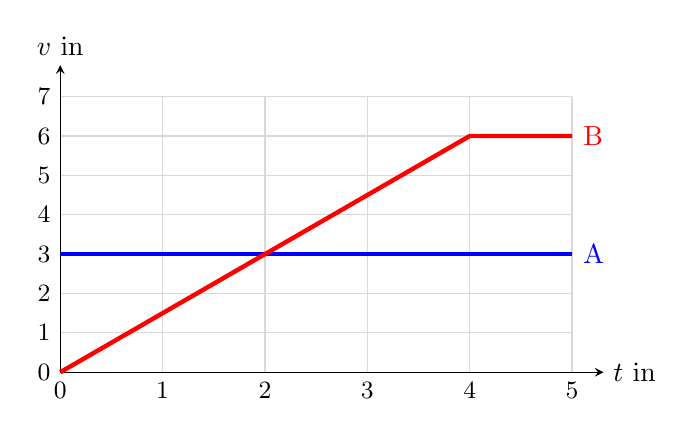
\begin{tikzpicture}[>=stealth, x=1.3cm, y=0.5cm]
 \draw[gray!30] (0,0) grid[xstep=1, ystep=1] (5,7);
 \draw[->] (0,0) -- (5.308,0) node[right] {$t$ in \si{\second}};
 \draw[->] (0,0) -- (0,7.8) node[above] {$v$ in \si{\meter\per\second}};
 \foreach \tk in {0,1,2,3,4,5} \node[below] at (\tk,0) {\small $\tk$};
 \foreach \yk in {0,1,2,3,4,5,6,7} \node[left] at (0,\yk) {\small $\yk$};

 \draw[ultra thick, blue] (0,3) -- (5,3) node[right] {A};
 \draw[ultra thick, red] (0,0) -- (4,6) -- (5,6) node[right] {B};
\end{tikzpicture}
\end{center}
\begin{abcliste}
\abc Welches Fahrzeug ist zur Zeit $t = \tCO$ schneller?
\abc Welches ist zur Zeit $t = \tCO$ weiter vorne? Wie weit sind beide gefahren?
\abc Wann holt B das Fahrzeug A ein?
\end{abcliste}
